%Accurate simulations of all stages of the production process is of crucial importance to make decisions aimed to speed up the performance improvement of a shop floor. 
%Applying discrete simulation techniques to a traditional shop floor can be a resource and time consuming process mainly due to data inaccuracies as even small variations of production parameters might lead to divergent simulation results compared to the actual system.

%In the industry 4.0 context, the shop floor is made by self-monitoring production machines and robots, namely CPS, with the capability to share their own state information with other stakeholders. Through a connection layer, this information can be exchanged and stored and used for achieving more realistic simulation input data which, in turn, leads to more accurate forecasting capabilities. In this way, the factory behavior can be accurately predicted in advance. Moreover, thanks to this quasi real-time mirroring of real elements into their virtual representation, it is possible to simulate on current data thus exploiting simulation potentials not only in the factory design and planning phase but also in the operative one. This allows to perform what-if analysis on the current production situation in order to support decision-making processes aimed at improving performances typically outside the boundaries of simulation such as ensuing the on-time delivery of customer orders or reallocating production resources to balance the current production.


In the FAR-EDGE Architecture (Figure~\ref{fig:r2ds}) several technological tiers are foreseen (from Field to Cloud) and the \textit{Real-to-Digital Synchronization} component is located in the uppermost tier, the Cloud Tier. Nevertheless, this component must also work closely with the other elements of the architecture to fulfill its role. Schematically (and referring only to the process of updating the digital twins stored in the \textit{Model Repository}), the Real-to-Digital Synchronization component must be able to access the services offered by the Edge layer and this is accomplished by means of the use of a system data bus. 

\begin{figure}[t]
  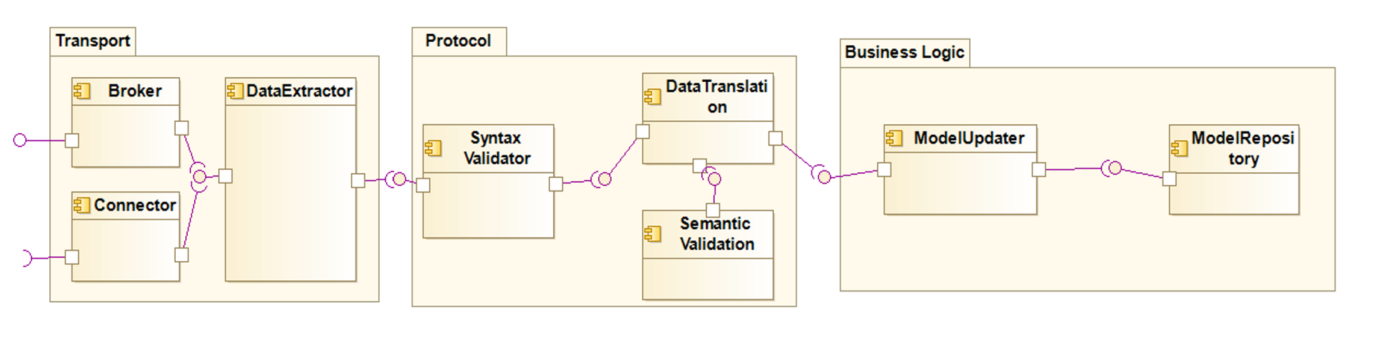
\includegraphics[width=\linewidth]{images/diagramComponent.PNG}
  \caption{Real to Digital Synchronization Component Diagram}
  \label{fig:realToDigitalComponentDia}
\end{figure}

Figure~\ref{fig:realToDigitalComponentDia} details the internal elements of the Real to Digital Synchronization component. 
Three main units interact to carry out the synchronization process, namely:
\begin{description}
\item The \textbf{Data Client}, which is the component in charge of bridging the physical to the digital world. Specifically, the main objective of this component is to provide access to the data produced in the Field tier. This is achieved in two ways:
\begin{enumerate}
\item The first way is to access the data through a registered broker in a \textit{PUSH} mode, meaning that the client is notified if new data is available.
\item The second way is to send a request using a client named in Figure~\ref{fig:realToDigitalComponentDia} as \textbf{Connector} in a \textit{PULL} mode, meaning that the client is responsible for asking if new data is available. An example of Connector can be a HTTP Client.
\end{enumerate}
Both the data connection modes communicate with the \textbf{Data Extractor} component, which is responsible for eliciting the information sent through the communication channel. 
The output of this component is a pure SenML~\cite{jennings2018sensor} data structure. SenML is a specification to define sensor measurement and it provide the possibility of being represented by different formats including XML and JSON. The SenML excerpt in Figure~\ref{fig:senML} represents the sensor reading of an item that has just been produced and informs the transport process to store the it in the warehouse. In addition to the name of the sensor and the timestamp of the measurement, in the message, other information are provided such as the serial number and the production line where the product has been assembled.

\begin{figure}[h]
  \frame{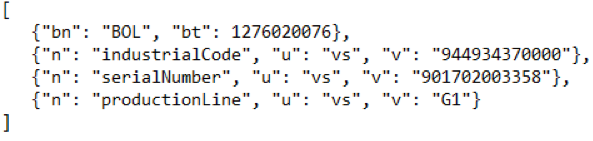
\includegraphics[width=0.7\linewidth]{images/senMl.png}}
  \caption{Example of message in SenML format}
  \label{fig:senML}
\end{figure}

The main advantage of this approach is that the underlying technologies responsible for communicating the message can be decoupled from the content of the message itself. 
By replacing the particular broker or connector, indeed, the component can be adapted to any communication protocol. 
%A prototype of this component is available in the Test Environment that is presented in Section \textbf{XXXX} In that version, the Data Client uses a subscription to a Kafka Channel that provides the functionalities of Broker and \textit{DataExtractor}.

\item The \textbf{Format Manager}, which is responsible for managing the data format. Since in the project vision each CPS vendor will be responsible for defining the message format, both semantically and syntactically, a specific component able to deal with conversion issues is required.
This component receives from the \textit{Data Client} a message containing the incoming serialized information from the shop floor. 
This message undergoes a first syntax check using a specific JSON-schema performed by the \textbf{Syntax Validator}. 
Afterwards, the whole message is parsed by the \textbf{Data Translator}, where a second check about the semantics is performed. 
Finally, the information is translated into an internal format required by the next component of the architecture. 

\item The \textbf{Business Logics Manager}, which is responsible for organizing the data in the Simulation \textit{Model Repository}. The main responsibility of this component is to map the data contained in the sensor message with the specific data model instantiated in the model repository component.
After the message parsing phase, the shop floor data is validated and is available for the comparison with the corresponding model repository data.
\end{description}



The remainder of this section details the interactions among the aforementioned. In the sequence diagrams shown in Figure~\ref{fig:r2dssequence} the overall real to digital synchronization workflow is presented.
The initial step in order to align the platform with the available sensor data is to connect it to the shop floor. 
The platform receives from the Monitoring App, through a \textit{PlatformCommandHandler} the \textit{ConnectPlatform} message. 
This causes a request to the \textit{FaredgeAPI} (that abstracts the interface with the architecture) which returns the list of active CPS.
For each CPS that is found, its specific configuration is loaded. The configuration specify if a synchronization model is associated with the particular CPS.  In case of a positive response, the platform instantiates a synchronization component, connects it to the CPS data sources and executes the model. Thereinafter all the active CPS are subscribed to the data bus topic, and can send their own sensor data.


\begin{sidewaysfigure}
  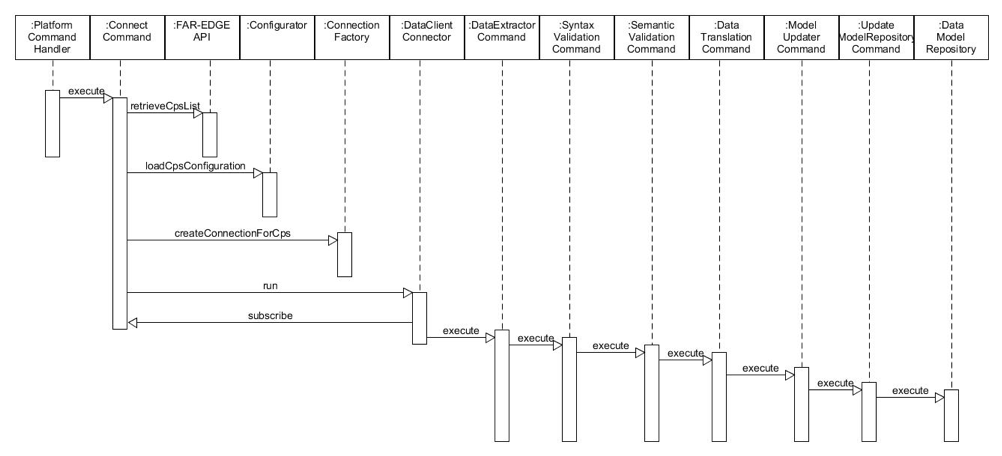
\includegraphics[width=\textheight]{images/R2DSsequence.png}
  \caption{Real-to-Digital Synchronization process - Sequence Diagram}
  \label{fig:r2dssequence}
\end{sidewaysfigure}


When a CPS communicates new sensor data, the \textit{DataClientConnector} is invoked. Its main responsibility is to activate the \textit{DataExtractor}; this reads the topic and the sensor data from the communication channel and forwards them to the \textit{SyntaxValidator}.
During this step the message is verified using the appropriate JSON schema. If the data format is recognized, a second validation is made. In this phase the values are checked in order to ensure the semantic quality of the data.
Upon successful completion of the second validation, the sensor data are sent to the \textit{DataTranslator}. This component provides a translation into a common internal format. After this step the message is totally decoupled from its original format. That allows to use different data formats, potentially one for each CPS. 


The virtualization and simulation platform has been developed and tested in a laboratory environment with particular reference to the case study presented in the next section. Notably, in addition to the components just described, a web application for graphical monitoring has been created that allows the user to manage the system remotely. Figure~\ref{fig:wizard} shows a screenshot of this application. 
In order to allow any vendor to create their own implementations of real to digital, a graphical interface has been developed in the project. 
By means of a wizard, this graphical interface allows the user to manage the behaviour of that component. 
Three main functionalities are exposed
\begin{description}


\item \textbf{Download Archetype}: In this step, the person responsible for the real-to-digital of a CPS can download a Archetype containing the framework classes needed to implement the CPS digital twin and the synchronization process. The package also contains the parsing libraries to streamline the developing and testing processes.
\item \textbf{Upload}: Once the component development is complete, the user can upload the CPS digital twin to the platform.
\item \textbf{Pairing}: This interface shows the list of CPS currently connected to the platform along with their synchronization models (if available). The user can manually pair the CPS with the model. It is possible to associate a different model to each CPS or reuse an existing one according to the use case.
\item \textbf{Activation}: At this point the CPSs connected to the platform are associated with the real to digital drivers. As the last step is just to activate the CPS so as to allow the connection and start receiving the synchronization of data. The CPS can be deactivated at any time in order to allow, for example, updates to the synchronization models.
\end{description}

\begin{figure}
  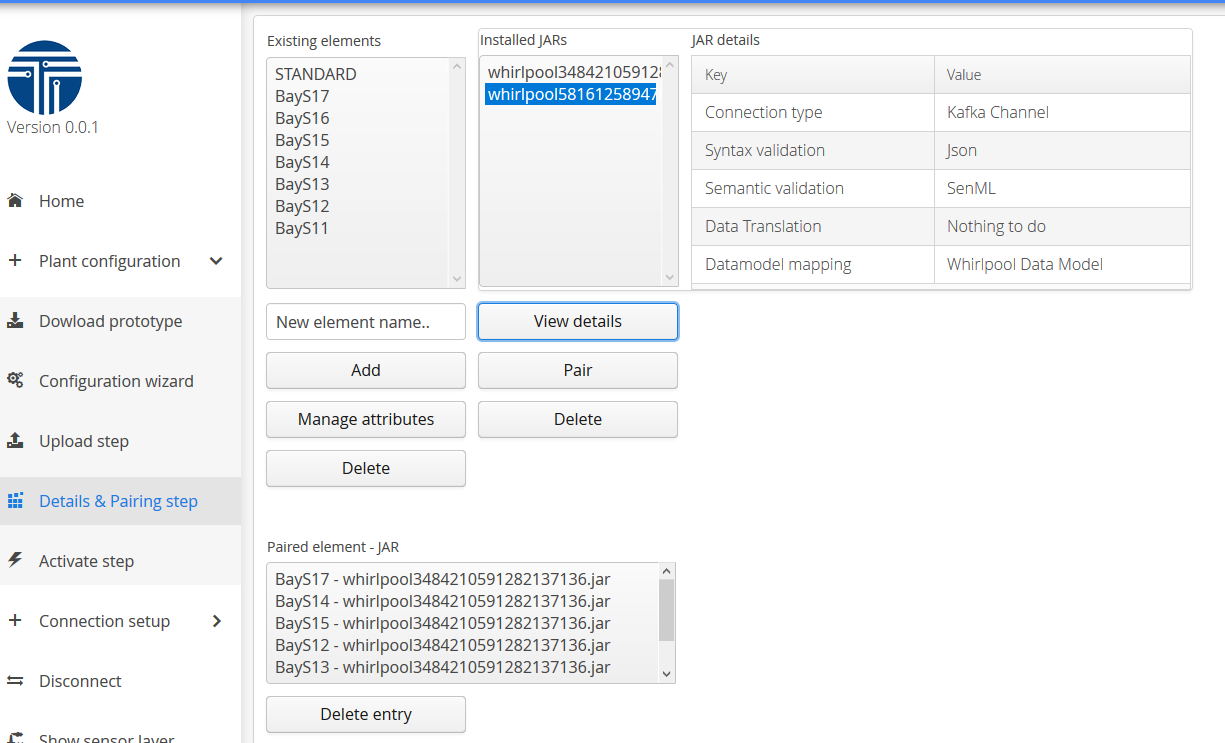
\includegraphics[width=\linewidth]{images/wizard.PNG}
  \caption{Real to Digital Synchronization wizard}
  \label{fig:wizard}
\end{figure}





